% Schematic of the OECD inter-country input-output (ICIO) table, drawn in TikZ
% (replaces the former OECD_table.png). Input from draftPaper.tex.
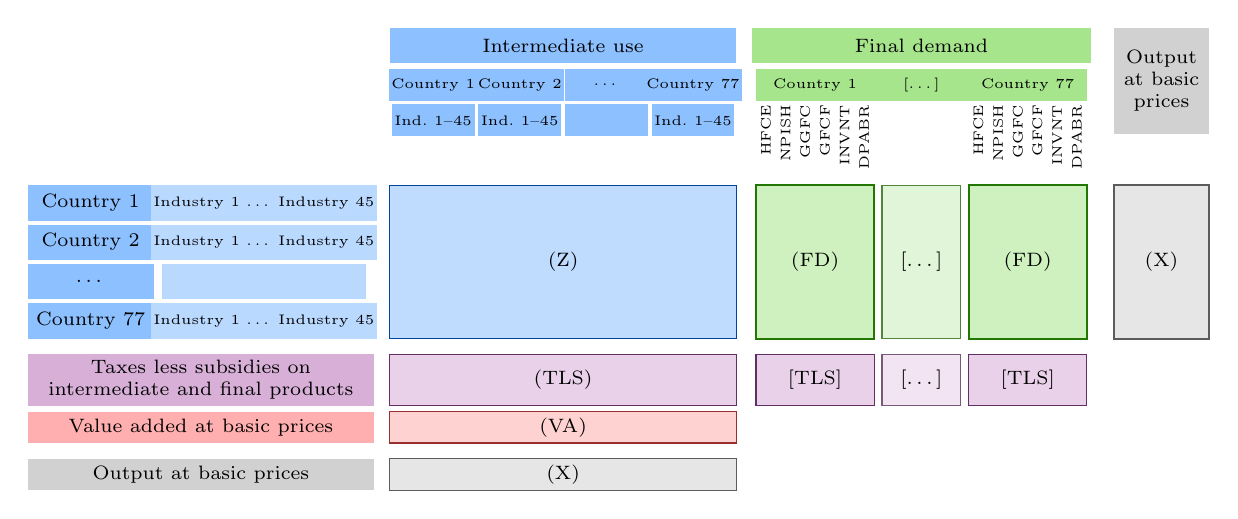
\begin{tikzpicture}[x=1cm, y=1cm, font=\scriptsize,
    blk/.style={draw=#1!60!black, fill=#1!25, line width=0.4pt, inner sep=1pt, align=center},
    hdr/.style={fill=#1!45, inner sep=1pt, align=center},
    sub/.style={fill=#1!45, inner sep=1pt, align=center, font=\tiny}]
  \colorlet{icioblue}{blue!55!cyan}
  \colorlet{iciogreen}{green!55!olive}
  \colorlet{iciopurple}{violet!70}
  \colorlet{iciored}{red!70}
  \colorlet{iciogrey}{black!40}
  \colorlet{icioblueL}{icioblue!60}
  \colorlet{iciogreenL}{iciogreen!60}
  \colorlet{iciopurpleL}{iciopurple!60}
  % ---- column headers ------------------------------------------------------
  \node[hdr=icioblue, minimum width=4.4cm, minimum height=0.45cm] at (6.8, 0) {Intermediate use};
  \node[hdr=iciogreen, minimum width=4.3cm, minimum height=0.45cm] at (11.35, 0) {Final demand};
  \node[hdr=iciogrey, minimum width=1.2cm, minimum height=1.35cm, align=center] at (14.4, -0.45) {Output\\at basic\\prices};
  % intermediate-use sub-headers: countries and industries
  \foreach \x/\t in {5.15/Country 1, 6.25/Country 2, 7.35/\dots, 8.45/Country 77} {
    \node[sub=icioblue, minimum width=1.05cm, minimum height=0.4cm] at (\x, -0.5) {\t};}
  \foreach \x in {5.15, 6.25, 8.45} {
    \node[sub=icioblue, minimum width=1.05cm, minimum height=0.4cm] at (\x, -0.95) {Ind.\ 1--45};}
  \node[sub=icioblue, minimum width=1.05cm, minimum height=0.4cm] at (7.35, -0.95) {};
  % final-demand sub-headers: countries and demand components (rotated)
  \foreach \x/\t in {10.0/Country 1, 11.35/{[\dots]}, 12.7/Country 77} {
    \node[sub=iciogreen, minimum width=1.5cm, minimum height=0.4cm] at (\x, -0.5) {\t};}
  \foreach \x in {10.0, 12.7} {
    \foreach \i/\c in {1/HFCE, 2/NPISH, 3/GGFC, 4/GFCF, 5/INVNT, 6/DPABR} {
      \node[rotate=90, font=\tiny, inner sep=0pt, anchor=east] at (\x - 0.75 + 0.25*\i - 0.125, -0.75) {\c};}}
  % ---- row headers ---------------------------------------------------------
  \foreach \y/\t in {-2.0/Country 1, -2.5/Country 2, -3.0/\dots, -3.5/Country 77} {
    \node[hdr=icioblue, minimum width=1.6cm, minimum height=0.45cm] at (0.8, \y) {\t};}
  \foreach \y in {-2.0, -2.5, -3.5} {
    \node[sub=icioblueL, minimum width=2.6cm, minimum height=0.45cm] at (3.0, \y) {Industry 1 \dots\ Industry 45};}
  \node[sub=icioblueL, minimum width=2.6cm, minimum height=0.45cm] at (3.0, -3.0) {};
  % ---- body blocks ---------------------------------------------------------
  \node[blk=icioblue, minimum width=4.4cm, minimum height=1.95cm] at (6.8, -2.75) {(Z)};
  \node[blk=iciogreen, minimum width=1.5cm, minimum height=1.95cm, line width=0.8pt] at (10.0, -2.75) {(FD)};
  \node[blk=iciogreenL, minimum width=1.0cm, minimum height=1.95cm] at (11.35, -2.75) {[\dots]};
  \node[blk=iciogreen, minimum width=1.5cm, minimum height=1.95cm, line width=0.8pt] at (12.7, -2.75) {(FD)};
  \node[blk=iciogrey, minimum width=1.2cm, minimum height=1.95cm, line width=0.8pt] at (14.4, -2.75) {(X)};
  % ---- bottom rows ---------------------------------------------------------
  \node[hdr=iciopurple, minimum width=4.4cm, minimum height=0.65cm, align=center] at (2.2, -4.25)
    {Taxes less subsidies on\\intermediate and final products};
  \node[blk=iciopurple, minimum width=4.4cm, minimum height=0.65cm] at (6.8, -4.25) {(TLS)};
  \node[blk=iciopurple, minimum width=1.5cm, minimum height=0.65cm] at (10.0, -4.25) {[TLS]};
  \node[blk=iciopurpleL, minimum width=1.0cm, minimum height=0.65cm] at (11.35, -4.25) {[\dots]};
  \node[blk=iciopurple, minimum width=1.5cm, minimum height=0.65cm] at (12.7, -4.25) {[TLS]};
  \node[hdr=iciored, minimum width=4.4cm, minimum height=0.4cm] at (2.2, -4.85) {Value added at basic prices};
  \node[blk=iciored, minimum width=4.4cm, minimum height=0.4cm] at (6.8, -4.85) {(VA)};
  \node[hdr=iciogrey, minimum width=4.4cm, minimum height=0.4cm] at (2.2, -5.45) {Output at basic prices};
  \node[blk=iciogrey, minimum width=4.4cm, minimum height=0.4cm] at (6.8, -5.45) {(X)};
\end{tikzpicture}
